\chapter{PLANTEAMIENTO DEL PROBLEMA}
\section{Descripción de la Realidad Problemática}

El cobre, cuyo símbolo es Cu, se caracteriza por ser un elemento metálico maleable, dúctil y también un excelente conductor de calor y electricidad. Este metal se encuentra en nuestro planeta de forma natural en distintas formas. Se puede hallar en diferentes depósitos de minerales y en estado puro o dicho de otra forma «nativo» \parencite{cu_internationalcopper2018}. Esto último, es lo que lo vuelve un mineral atractivo, además de, una vez convertido en un producto terminado por las industrias, este puede ser empleado en el sector automovilístico, sector eléctrico, productos electrónicos, tecnologías de comunicación, construcciones, maquinaria industrial  y otros artículos de la vida cotidiana. %\medskip



\begin{figure}[h]
	\begin{center}
		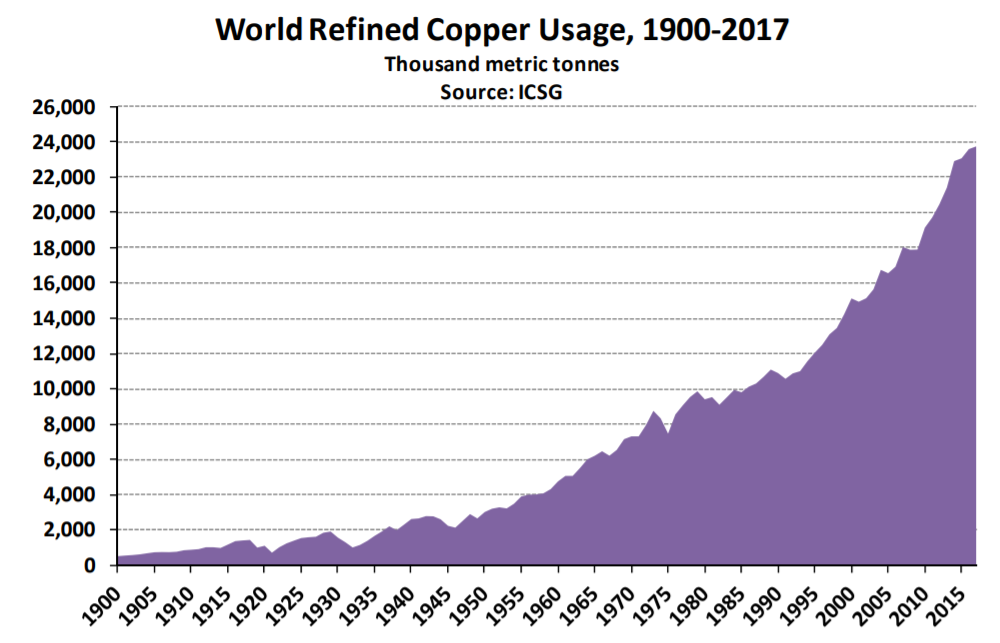
\includegraphics[width=0.8\textwidth]{1/figures/world_refined_copper_usage.png}
		\caption{Uso del cobre refinado mundial del año 1900 a 2017 (en miles de toneladas). Fuente: \cite{cu_internationalcopper2018}}
		\label{1:fig}
	\end{center}
\end{figure}

A lo largo de los años, como se observa en la Figura \ref{1:fig}, el uso del cobre refinado (cobre de alta pureza con una concentración de 99.9\%) en el mundo ha tenido un incremento bastante significativo y ello ha conllevado a un aumento en la comercialización de dicho metal. Como consecuencia, este ha contribuido en gran medida para las economías de diversas naciones ya sean países maduros o en vías de desarrollo. El minado, procesamiento, reciclaje y transformación de este metal a varios productos ha creado trabajos y generado riqueza. Estas actividades contribuyen en construir y mantener la infraestructura de un país, y además crea oportunidades de comercio e inversión \parencite{cu_internationalcopper2018}.



\begin{figure}[h]
	\begin{center}
		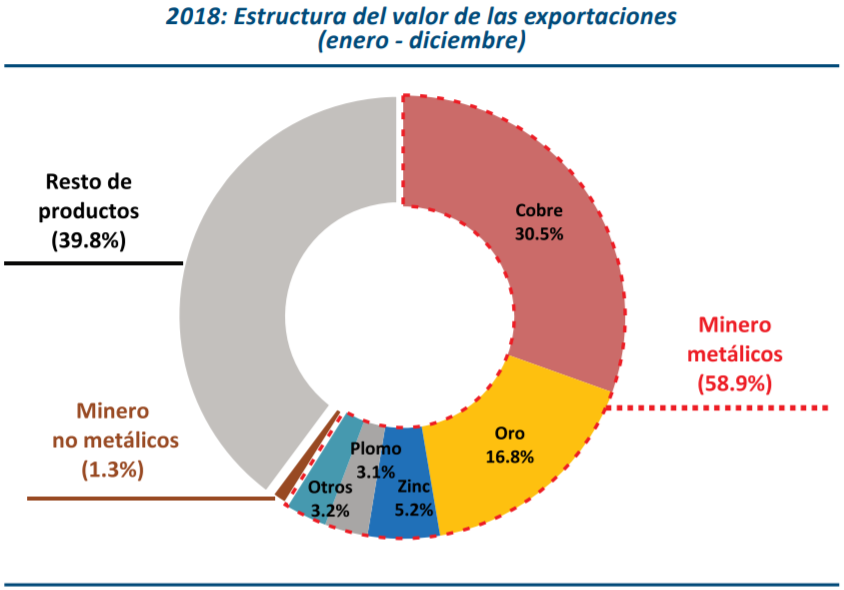
\includegraphics[width=0.8\textwidth]{1/figures/estructura_exportaciones_peru.png}
		\caption{Estructura del valor de las exportaciones peruanas en el año 2018. Fuente: \cite{cu_ministerioPeru_statsminas}}
		\label{1:fig2}
	\end{center}
\end{figure}




\begin{figure}[h]
	\begin{center}
		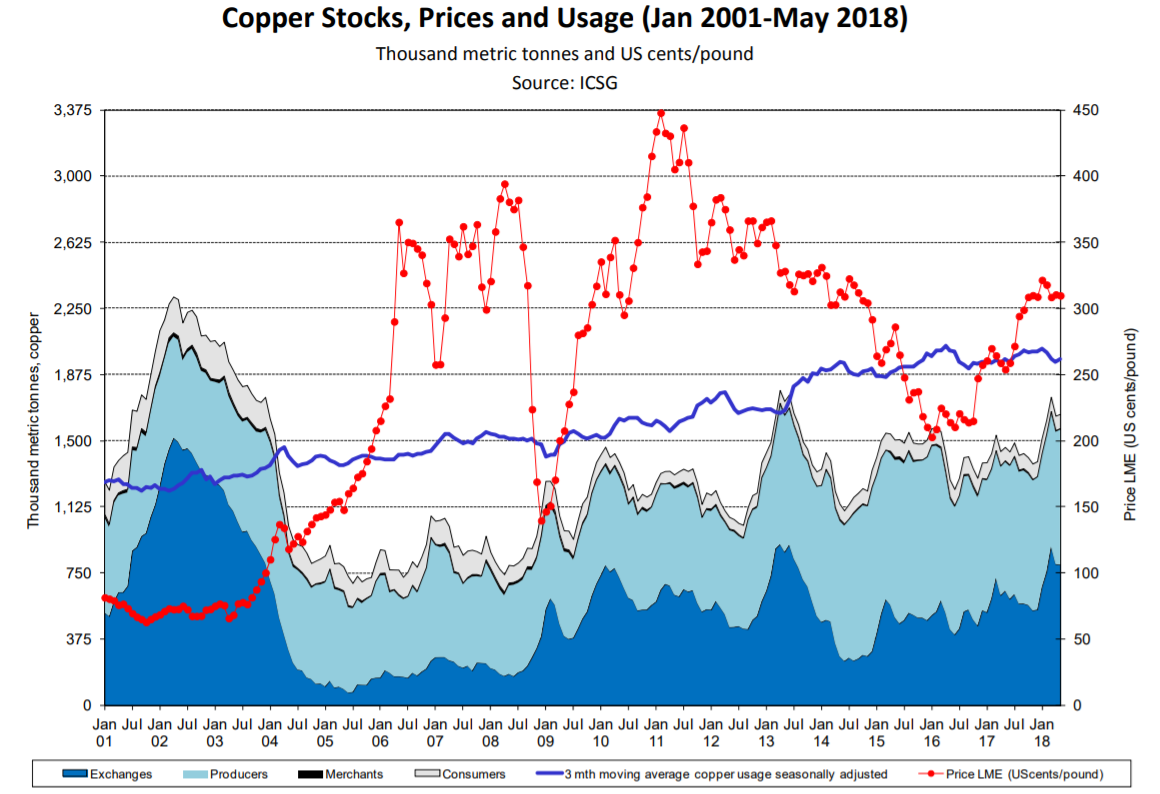
\includegraphics[width=0.8\textwidth]{1/figures/copper_stocks_prices_usage.png}
		\caption{Precio, stocks y uso del cobre (cantidad en miles de toneladas y precio en centavos por libra). Fuente: \cite{cu_internationalcopper2018}}	
		\label{1:fig3}
	\end{center}
\end{figure}

Estos modelos usados para predecir precios se basan mayormente en estimaciones de la oferta y demanda futura, así como los inventarios de bolsa. Otros consideran la memoria histórica de estas variables, la información de costos futuros de proyectos mineros, o variables financieras. Sin embargo, lo que estos modelos no hacen, es predecir el momento de la caída o alza del precio debido a eventos que no dependen de ninguna de las variables antes mencionadas sino a hechos inesperados globales \citep{cu_lagos2017proyectar}. 


\begin{figure}[h]
	\begin{center}
		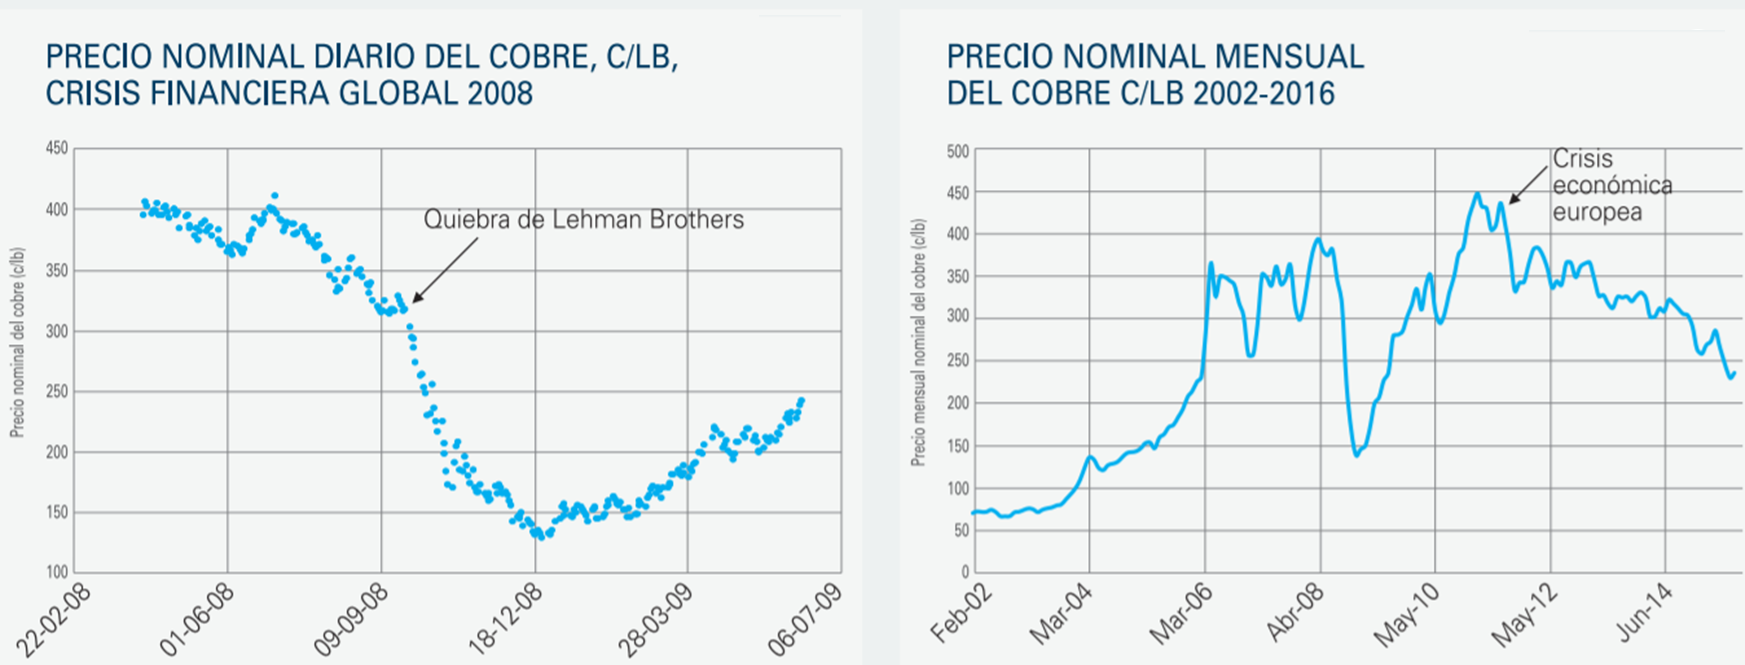
\includegraphics[width=0.8\textwidth]{1/figures/precio_caidas_gustavo_lagos.png}
		\caption{Precio, stocks y uso del cobre (cantidad en miles de toneladas y precio en centavos por libra). Fuente: \cite{cu_lagos2017proyectar}}
		\label{1:fig4}
	\end{center}
\end{figure} 




\section{Formulación del Problema}

Para lefecto \parencite{ot_marti2018manual}. 


Una vez elaborado el diagrama (véase Anexo 1), 

\subsection{Problema General}
\newcommand{\ProblemaGeneral}{
	El incremento del fraude en Perú mediante el uso de tecnologías deepfake de audio ha evidenciado la falta de herramientas adecuadas para detectar estos fraudes, especialmente en español. Las técnicas actuales no logran identificar eficazmente las características acústicas del español, como el tono de voz, timbre de voz, patrones de voz, frecuencia fundamental (pitch), duración y ritmo del habla, formantes, nivel de energía del habla (intensidad), ruidos de fondo, prosodia, articulación y transiciones entre fonemas, lo que facilita la suplantación de identidad y el fraude en las comunicaciones personales y empresariales. 
}
\ProblemaGeneral
\subsection{Problemas Espec\'{i}ficos}
\newcommand{\Pbone}{
La falta de un dataset en español que incluya variaciones regionales y voces manipuladas dificulta el entrenamiento de modelos de redes neuronales profundas para detectar deepfakes de audio en español, debido a las diferencias en patrones de voz, frecuencia fundamental (pitch) y ritmo del habla.
}
\newcommand{\Pbtwo}{
Las técnicas actuales no logran detectar las variaciones en el tono de voz, timbre de voz y formantes en audios en español, lo que disminuye la precisión en la identificación de audios manipulados.
}
\newcommand{\Pbthree}{
Los fraudes por suplantación de identidad mediante deepfakes de audio en Perú son difíciles de detectar con las técnicas actuales debido a la falta de análisis de prosodia, articulación, transiciones entre fonemas y ruidos de fondo, lo que incrementa el riesgo de fraude.
}


\begin{itemize}
	\item \Pbone
	\item \Pbtwo
	\item \Pbthree

\end{itemize}

\section{Objetivos de la Investigación}
Para la formulación de los objetivos de la presente investigación se elaboró un «árbol de objetivos» (véase Anexo 2) 
\subsection{Objetivo General}
\newcommand{\ObjetivoGeneral}{
Desarrollar un modelo basado en redes neuronales profundas que permita detectar deepfakes de audio en español mediante el análisis de variables clave como tono de voz, timbre de voz, patrones de voz, frecuencia fundamental, duración y ritmo del habla, formantes, nivel de energía del habla, ruidos de fondo, prosodia, articulación y transiciones entre fonemas, mejorando la precisión en la identificación de audios manipulados para mitigar fraudes por suplantación de identidad en Perú.
}
\ObjetivoGeneral
\subsection{Objetivos Espec\'{i}ficos}
\newcommand{\Objone}{
Desarrollar un dataset específico en español, con variaciones regionales y voces manipuladas, para entrenar un modelo de redes neuronales profundas que detecte deepfakes de audio
}
\newcommand{\Objtwo}{
Implementar un modelo de redes neuronales profundas que analice el tono de voz, timbre de voz y formantes para mejorar la precisión en la detección de deepfakes de audio en español.
}
\newcommand{\Objthree}{
Evaluar la eficacia del modelo de redes neuronales profundas en la detección de deepfakes de audio en contextos de fraude por suplantación de identidad en Perú, considerando prosodia, articulación, transiciones entre fonemas y ruidos de fondo.
}

\begin{itemize}
	\item {\Objone}
	\item {\Objtwo}
	\item {\Objthree}
\end{itemize}

\section{Justificación de la Investigación}

\subsection{Teórica}
Esta investigación se realiza 

\subsection{Práctica}
Al culminar la investigación 

\subsection{Metodológica}. 

\section{Delimitación del Estudio}

\subsection{Espacial}
Para la presente investigación 

\subsection{Temporal}
Los datos que serán necesari. 

\subsection{Conceptual}
Esta investigación se 

\section{Hipótesis}

\subsection{Hipótesis General}
\newcommand{\HipotesisGeneral}{
El uso de un modelo basado en redes neuronales profundas que analice las variables acústicas clave como tono de voz, timbre de voz, patrones de voz, frecuencia fundamental, duración y ritmo del habla, formantes, nivel de energía del habla, ruidos de fondo, prosodia, articulación y transiciones entre fonemas mejora significativamente la precisión en la detección de deepfakes de audio en español, reduciendo el riesgo de fraudes por suplantación de identidad en Perú.
}
\HipotesisGeneral
\subsection{Hipótesis Específicas}
\newcommand{\Hone}{
La creación de un dataset en español que incluya variaciones regionales y voces manipuladas mejorará significativamente la capacidad de las redes neuronales profundas para detectar deepfakes de audio en este idioma
}
\newcommand{\Htwo}{
El análisis del tono de voz, timbre de voz y formantes mediante redes neuronales profundas aumentará la precisión en la detección de deepfakes de audio en español.
}
\newcommand{\Hthree}{
El modelo de redes neuronales profundas será más efectivo en la detección de deepfakes en contextos de fraude en Perú al incluir el análisis de prosodia, articulación, transiciones entre fonemas y ruidos de fondo, en comparación con las técnicas actuales.	
}

\begin{itemize}
	\item \Hone
	\item \Htwo
	\item \Hthree
\end{itemize}

\subsection{Matriz de Consistencia}
A continuación se presenta la matriz de consistencia elaborada para la presente investigación (véase Anexo \ref{1:table}).

